\begin{frame}
    \frametitle{Optimization Tool's Design Goals}
    \begin{minipage}[c]{0.45\textwidth}
    \begin{itemize}
        %\item ROLLO (Reactor evOLutionary aLgorithm Optimizer) is a Python package 
        %that applies evolutionary algorithms to optimize nuclear reactor design
        \item It couples an evolutionary algorithm driver, Distributed 
        Evolutionary Algorithms in Python (DEAP), with 
        nuclear software, such as neutron transport OpenMC and thermal-hydraulics 
        Moltres codes
        \item Design Goals: effective, flexible, open-source, parallel,
        reproducible
    \end{itemize}
    \end{minipage}\hfill
    \begin{minipage}[c]{0.55\textwidth}
        \centering
        \begin{figure}
            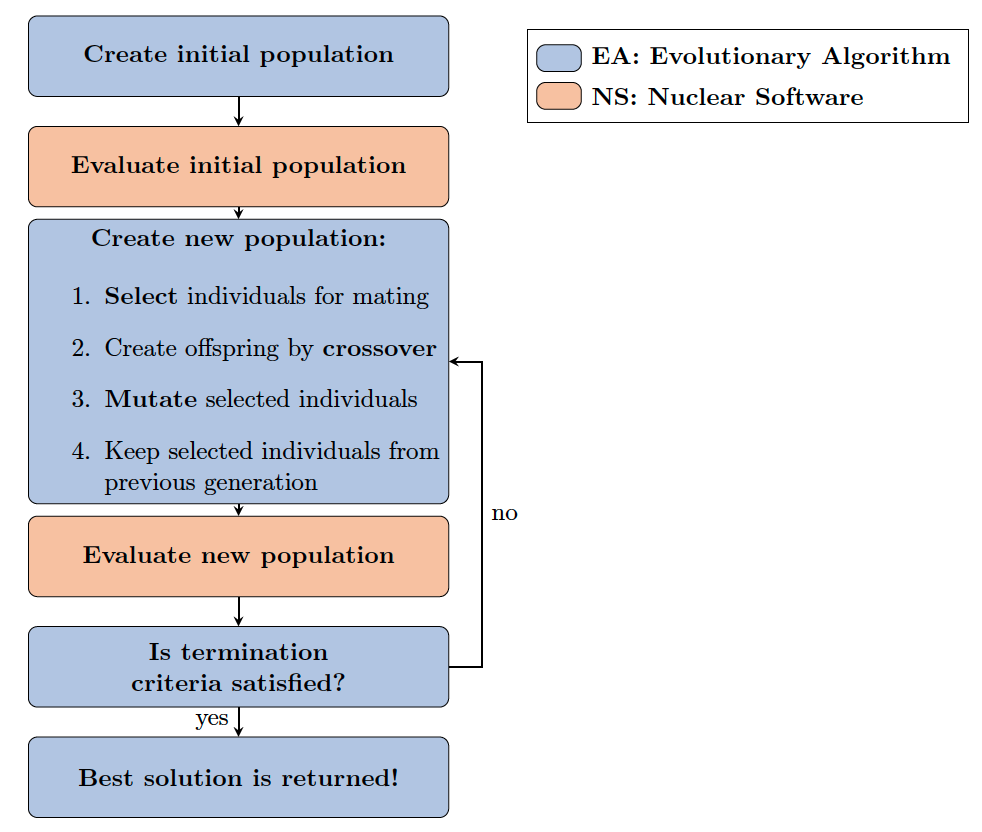
\includegraphics[width=\linewidth]{figures/rollo-flow.png} 
            \caption{Optimization tool's flow.}
        \end{figure}
    \end{minipage}
    %\begin{block}{ROLLO Design Goals}
    %    \begin{itemize}
    %        \item Effective: good documentation, well tested, version controlled 
    %        on Github 
    %        \item Flexible: user can vary any imaginable parameter because
    %       ROLLO uses a templating method to edit the input file of the coupled software.
    %        \item Open-source: utilizes only open-source dependencies 
    %        \item Parallel: toggle to enable parallelization on local and HPCs
    %        \item Reproducible: Data from every ROLLO run saves into a unique, 
    %        pickled file (pickle is a Python module that serializes Python 
    %        objects), and all results from this work are available on Github.
    %    \end{itemize}
    %\end{block}
\end{frame}